\section{Bluetooth}

\begin{figure}[H]
\begin{center}
	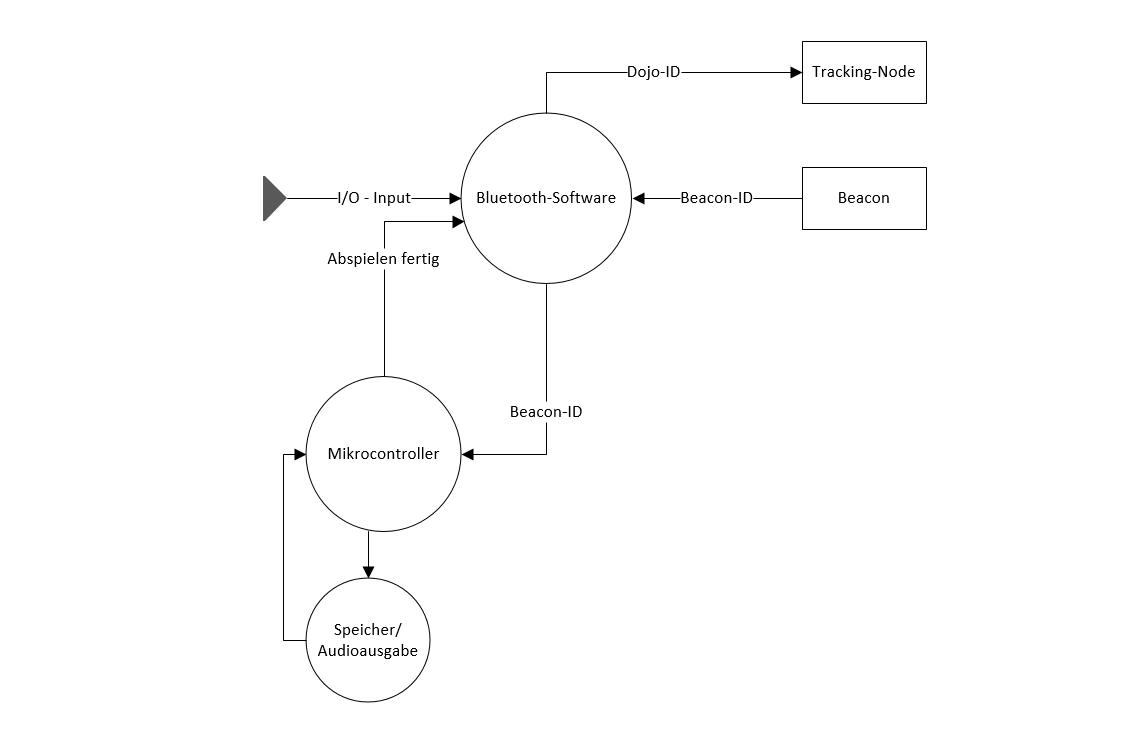
\includegraphics[width=120mm]{data/Bluetooth.png}
	\caption{Grobstruktur der Bluetooth-Software} %picture caption
	\label{fig:bluetooth_grobstruktur}
\end{center}
\end{figure}

Obenstehende Abbildung zeigt die Grobstruktur der Bluetooth-Software. Über die Software erfolgt ein Input (Software – Input), welche das Suchen von Bluetooth Signalen in der Nähe auslöst. Vom Beacon mit dem stärksten Signal wird dann die Beacon-ID empfangen. Diese Beacon-ID wird Software-intern weitergeleitet, um das zugehörige Audio-File abzuspielen. Während des Abspielens der Audio-Datei ist das weitere Suchen deaktiviert, um Überschneidungen von Programmabläufen und daraus resultierende mögliche Fehler zu minimieren. Nach dem Abspielen einer Audio-Datei wird das Suchen wieder ermöglicht. Für ein mögliches Einbinden des Dojo in ein Tracking-System wird der Dojo in der Lage sein, seine eigene Erkennungsnummer auf Anfrage zu senden, ähnlich wie ein Beacon. 
\subsection{Schnittstellen zu anderen Bereichen:}
Dojo soll, um Energie zu sparen, erst per Knopfdruck das Kunstobjekt mit der stärksten Signalstärke suchen und die entsprechende Datei dafür abspielen. Dies führt Software-intern zu einer Parameterübergabe an die Audio-/Speichersektion. Während der Audiowiedergabe soll das BT ausgeschaltet bleiben, weshalb wiederum Software-intern eine Parameterübergabe bzw. -Abfrage erfolgen muss. Dies soll verhindern, dass während der Audio-Wiedergabe das Suchen und Abspielen eines weiteren Objekts möglich ist. Beim Wunschziel Daten-Austausch herrscht eine enge Verbundenheit zwischen BT und Speicher. 
